\chapter{Problema de Roteamento de Veículos}\label{sec:vrp}

O Problema de Roteamento de Veículos (\textit{Vehicle Routing Problem} — VRP) é um dos problemas de otimização combinatória mais estudados na literatura, sendo frequentemente considerado uma generalização natural do Problema do Caixeiro Viajante (\textit{Travelling Salesman Problem} — TSP) \cite{gavish1978travelling}. Enquanto o TSP busca determinar a rota mínima para um único agente visitar um conjunto de cidades, o VRP introduz múltiplos veículos e um conjunto mais amplo de restrições operacionais, tornando-o mais adequado para modelar situações reais, o que aumenta significativamente a complexidade do problema.

De forma geral, o VRP pode ser descrito como o problema de determinar um conjunto de rotas para uma frota de veículos, partindo de um ou mais depósitos, de modo a atender um conjunto de clientes com demandas conhecidas, respeitando as restrições impostas e minimizando um critério de custo, usualmente associado à distância total percorrida ou ao tempo de operação. Cada cliente deve ser atendido exatamente uma vez, por exatamente um veículo, e todos os veículos devem retornar ao depósito de origem ao término de sua rota. A escolha de quais clientes serão atendidos por cada veículo, e em qual ordem, constitui o núcleo combinatório do problema, cuja formalização matemática será apresentada na seção seguinte. Uma ilustração do problema é apresentada na \autoref{fig:vrp}.

\begin{figure}[htbp]
    \centering
    \caption{Exemplo ilustrativo do VRP, no qual os clientes são distribuídos em rotas distintas, associadas a cinco diferentes veículos, com partida e retorno ao depósito central.}
    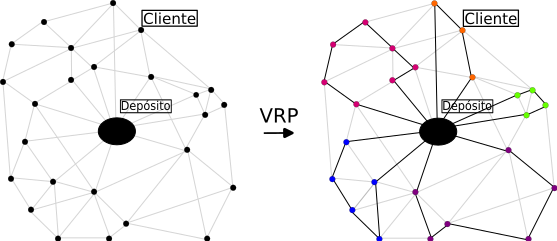
\includegraphics[width=.7\textwidth]{figs/vrp.png}
    \fonte{Autoria própria (2026)}
    \label{fig:vrp}
\end{figure}

O problema foi introduzido inicialmente no contexto de distribuição de combustível \cite{dantzig1959truck} e que vem acompanhando o desenvolvimento de métodos computacionais e técnicas de otimização. Houve avanços importantes na formulação matemática do problema especialmente com o uso de programação inteira. Posteriormente, devido a dificuldade computacional associada à sua natureza NP-Difícil \cite{hochba1997approximation}, a área passou a focar em propostas heurística e metaheurísticas capazes de encontrar soluções com boa qualidade em tempo de execução viável, dentre essas propostas podemos destacar: busca tabu \cite{glover1989tabu, glover1990tabu}, algoritmos genéticos \cite{boldberg1989genetic}, \textit{simulated annealing} \cite{kirkpatrick1983optimization} e colônia de formigas \cite{dorigo2002ant}. 

A relevância do VRP está diretamente relacionada ao seu amplo espectro de aplicações práticas. Problemas de roteamento são centrais em sistemas logísticos modernos, especialmente em contextos como distribuição urbana de mercadorias, coleta de resíduos, transporte escolar e planejamento de rotas para serviços de emergência \cite{golden2008vehicle,toth2002vehicle}. Além disso, com o avanço tecnológico, novas aplicações têm surgido, incluindo o roteamento de drones e veículos autônomos \cite{otto2018optimization}. Nessas aplicações, a eficiência das rotas impacta diretamente custos operacionais, consumo de combustível e emissões de gases poluentes \cite{lin2014survey}, tornando o VRP um problema de grande importância econômica e ambiental.

Ao longo do tempo, diversas variantes do VRP foram propostas para capturar diferentes aspectos do mundo real. Entre as mais estudadas, destacam-se o Problema de Roteamento de Veículos Capacitado (\textit{Capacitated VRP} - CVRP), no qual cada veículo possui uma capacidade limitada  \cite{solomon1987algorithms, xiao2012development}; o VRP com Janelas de Tempo (\textit{VRP with Time Window} - VRPTW), que considera restrições temporais para atendimento \cite{christofides1979vehicle, gambardella1999macs}; o VRP com Múltiplos Depósitos (\textit{Multi Depot VRP} - MDVRP) em que os veículos partem de diferentes depósitos para atender um conjunto de clientes da forma mais eficiente \cite{alinaghian2018multi}; e o VRP Estocástico, no qual parâmetros como demanda ou tempo de viagem são incertos \cite{renaud1996tabu, gendreau1996stochastic}. Essas variantes refletem a necessidade de modelos cada vez mais realistas e adaptados a cenários específicos.

Mais recentemente, novas tendências têm emergido na literatura, impulsionadas pela disponibilidade de dados em tempo real e pelo avanço de tecnologias como Internet das Coisas (\textit{Internet of Things} --- IoT) e sistemas de posicionamento global (\textit{Global Positioning System} --- GPS) \cite{ritzinger2016survey, boysen2018scheduling}. Nesse contexto, variantes dinâmicas do VRP têm ganhado destaque, permitindo a adaptação das rotas em tempo real. Além disso, há um crescente interesse em problemas de roteamento sustentáveis, como o VRP verde (Green VRP) \cite{lin2014survey} e o roteamento de veículos elétricos (\textit{Electric VRP} --- EVRP) \cite{schiffer2017electric}, que incorporam preocupações ambientais e restrições energéticas.

Dessa forma, o VRP permanece como um campo de pesquisa ativo e desafiador, com inúmeras aplicações práticas e diversas oportunidades para avanços metodológicos. A complexidade inerente ao problema, aliada à crescente demanda por soluções eficientes e sustentáveis, reforça sua relevância tanto do ponto de vista teórico quanto aplicado \cite{braekers2016vehicle, moghdani2021green}.

\section{Modelagem Matemática}

A Programação Linear Inteira (\textit{Integer Linear Programming} --- ILP) é uma das formulações exatas mais tradicionais para problemas de roteamento, sendo a base sobre a qual se constroem tanto os métodos de solução exata quanto as referências de qualidade para abordagens heurísticas \cite{toth2002vehicle, balas1983branch}. No contexto do VRP, o problema é modelado por meio de variáveis binárias que indicam se determinado arco entre dois nós é utilizado por algum veículo \cite{laporte1992vehicle}. Essa representação exige a inclusão de restrições de conservação de fluxo e de eliminação de sub-rotas para garantir a validade das soluções \cite{miller1960integer, desrochers1991improvements}, consolidando o uso de algoritmos exatos para lidar com as restrições de capacidade da frota \cite{baldacci2010exact, baldacci2010exact}.

Considere um grafo completo\footnote{Um \textit{grafo completo} é aquele em que todo par de vértices distintos está conectado por uma aresta.} $G = (V, E)$, onde $V = \{0, 1, \ldots, n\}$ \cite{applegate2011traveling} representa o conjunto de vértices, sendo $0$ o depósito e os demais nós correspondentes aos clientes, e $E$ o conjunto de arcos possíveis. A cada arco $(i,j) \in E$ associa-se um custo $c_{ij}$, usualmente interpretado como a distância ou o tempo de deslocamento entre os nós $i$ e $j$. O objetivo geral do VRP consiste em determinar um conjunto de rotas para uma frota de veículos $K$ \cite{dantzig1959truck}, partindo do depósito, de modo a atender todos os clientes exatamente uma vez e retornar ao depósito \cite{laporte2009fifty}, minimizando o custo total das rotas por meio de formulações matemáticas e algoritmos de otimização \cite{golden2008vehicle, desaulniers1998multi}.

Entre as variantes mais estudadas do VRP, destaca-se o Problema de Roteamento de Veículos Capacitado (\textit{Capacitated VRP} --- CVRP), no qual cada cliente $i \in V \setminus \{0\}$ possui uma demanda $d_i$ e cada veículo $k \in K$ dispõe de uma capacidade máxima $Q \in \mathbb{R}$, de modo que a soma das demandas atendidas em cada rota não pode exceder esse limite \cite{huang_solving_nodate}. Formalmente, define-se a variável de decisão binária

\begin{equation}
    x_{ijk} =
    \begin{cases}
        1, & \text{se o veículo } k \text{ percorre o arco } (i,j), \\
        0, & \text{caso contrário,}
    \end{cases}
    \label{eq:var_decisao}
\end{equation}

\noindent cuja função objetivo consiste em minimizar o custo total das rotas:

\begin{equation}
    \min \sum_{k \in K} \sum_{i \in V} \sum_{\substack{j \in V \\ j \neq i}} 
    c_{ij}\, x_{ijk}.
    \label{eq:fo_vrp}
\end{equation}

As restrições do modelo asseguram a viabilidade das rotas. A obrigatoriedade de visita a cada cliente exatamente uma vez é imposta por:

\begin{equation}
    \sum_{k \in K} \sum_{\substack{j \in V \\ j \neq i}} x_{ijk} = 1, 
    \quad \forall\, i \in V \setminus \{0\},
    \label{eq:visita_saida}
\end{equation}

\begin{equation}
    \sum_{k \in K} \sum_{\substack{i \in V \\ i \neq j}} x_{ijk} = 1, 
    \quad \forall\, j \in V \setminus \{0\}.
    \label{eq:visita_entrada}
\end{equation}

A \autoref{eq:visita_saida} garante que cada cliente é atendido por exatamente uma rota de saída \cite{clarke1964scheduling}, enquanto a \autoref{eq:visita_entrada} assegura que cada cliente é visitado exatamente uma vez por alguma rota de entrada \cite{toth2014vehicle}. Em conjunto, essas restrições impõem a conservação de fluxo nos nós correspondentes aos clientes \cite{Fisher1995}, evitando tanto visitas múltiplas quanto a omissão de clientes no conjunto de rotas.

A conservação de fluxo no depósito, que controla o número de veículos utilizados, é garantida por:

\begin{equation}
    \sum_{j \in V \setminus \{0\}} x_{0jk} = 1, \quad \forall\, k \in K,
    \label{eq:fluxo_saida}
\end{equation}

\begin{equation}
    \sum_{i \in V \setminus \{0\}} x_{i0k} = 1, \quad \forall\, k \in K.
    \label{eq:fluxo_entrada}
\end{equation}

As restrições de capacidade asseguram que a soma das demandas atendidas em cada rota não exceda a capacidade $Q$ do veículo:

\begin{equation}
    \sum_{i \in V} \sum_{\substack{j \in V \\ j \neq i}} d_j\, x_{ijk} \leq Q, 
    \quad \forall\, k \in K.
    \label{eq:capacidade}
\end{equation}

A presença dessa restrição de desigualdade, combinada às variáveis binárias $x_{ijk} \in \{0,1\}$ e às variáveis contínuas auxiliares $u_i \in \mathbb{R}$ \cite{miller1960integer}, caracteriza o modelo como um problema de Programação Linear Inteira Mista (\textit{Mixed Integer Linear Programming} --- MILP) \cite{Nemhauser1988}. Nessa classe de problemas, parte das variáveis de decisão assume valores inteiros ou binários, enquanto outra parte pode assumir valores reais \cite{Conforti2014}, o que aumenta significativamente a complexidade computacional em relação à ILP \cite{Wolsey1998}. Essa transição para modelos híbridos exige algoritmos especializados devido à natureza NP-difícil da busca por soluções ótimas em espaços discretos e contínuos simultâneos \cite{papadimitriou1998combinatorial}.

Além das restrições de visita, fluxo e capacidade, é necessário garantir a conectividade das rotas, impedindo a formação de sub-rotas desconectadas do depósito. A eliminação de sub-rotas constitui, portanto, um dos principais desafios na formulação matemática de problemas de roteamento de veículos, uma vez que as restrições básicas do modelo não são suficientes para assegurar a conectividade global das soluções \cite{dantzig1954solution}. Nesse contexto, diferentes estratégias de modelagem têm sido propostas na literatura, variando em complexidade e eficiência computacional \cite{Oncan2009}. Enquanto algumas abordagens utilizam variáveis de fluxo para projetar a conectividade \cite{Gouveia1995}, outras focam na adaptação de formulações clássicas para cenários de múltiplos veículos \cite{Bektas2006}. Independentemente do método, o objetivo central permanece garantir a viabilidade estrutural das rotas \cite{Achuthan1996}, respeitando as propriedades poliedrais que definem o espaço de soluções ótimas \cite{Letchford2006}.

Uma abordagem clássica consiste no uso de restrições explícitas de eliminação de sub-rotas \cite{dantzig2009solution}:

\begin{equation}
    \sum_{i \in S} \sum_{j \in S} x_{ijk} \leq |S| - 1, 
    \quad \forall\, S \subset V,\; 2 \leq |S| \leq |V| - 1,\; \forall\, k \in K,
    \label{eq:subciclo}
\end{equation}

\noindent em que $S$ representa qualquer subconjunto próprio de vértices que não inclui o depósito. A restrição impõe que o número de arcos selecionados dentro desse subconjunto seja estritamente menor que o necessário para formar um ciclo fechado, impedindo assim a ocorrência de sub-rotas desconectadas. Alternativamente, podem ser empregadas formulações baseadas em fluxo ou o uso de variáveis auxiliares, como na formulação de Miller--Tucker--Zemlin (MTZ) \cite{miller1960integer}, na qual $u_i$ representa a carga acumulada no momento da chegada ao nó $i$, e a variável binária $x_{ijk}$ indica se o veículo $k$ percorre o arco $(i,j)$, enquanto $d_j$ corresponde à demanda associada ao nó $j$. As restrições são dadas por:

\begin{equation}
    u_i - u_j + Q\, x_{ijk} \leq Q - d_j, 
    \quad \forall\, i \neq j,\; i,j \in V \setminus \{0\},\; \forall\, k \in K,
    \label{eq:mtz1}
\end{equation}

\begin{equation}
    d_i \leq u_i \leq Q, \quad \forall\, i \in V \setminus \{0\}.
    \label{eq:mtz2}
\end{equation}

Quando o arco $(i,j)$ é percorrido por algum veículo ($x_{ijk} = 1$), a restrição implica $u_j \geq u_i + d_j$, induzindo uma progressão ao longo da rota. Essa característica impede a formação de ciclos inconsistentes e contribui para a eliminação de sub-rotas, ao mesmo tempo em que assegura o respeito à capacidade $Q$.

O TSP pode ser interpretado como um caso particular do VRP no qual há um único veículo ($|K| = 1$) \cite{toth2002vehicle} e as restrições de capacidade são suprimidas, ou, equivalentemente, $Q$ é suficientemente grande para atender todos os clientes em uma única rota \cite{balinski1964integer, eilon1974distribution}. Nesse caso, as variáveis binárias $x_{ij}$ indicam se a aresta entre as cidades $i$ e $j$ pertence ao ciclo Hamiltoniano, e a formulação resultante preserva a mesma função objetivo com um conjunto reduzido de restrições, reduzindo o problema à determinação de um ciclo Hamiltoniano de custo mínimo, definido como o caminho fechado que percorre todos os vértices de um grafo exatamente uma vez, retornando ao vértice inicial ao final.

Embora a formulação por programação inteira seja conceitualmente direta, o número de restrições de eliminação de subciclos pode crescer exponencialmente com o tamanho da instância \cite{dantzig1954solution}, o que torna o uso direto dessa abordagem computacionalmente limitado para instâncias de grande porte. Ainda assim, modelos de programação inteira desempenham papel central na área, pois fornecem soluções ótimas garantidas, limites inferiores precisos e formulações de referência para avaliar a qualidade de métodos heurísticos e metaheurísticos, que serão discutidos na seção seguinte.